%%%%%%%%%%%%%%%%%%%%%%%%%%%%%%%%%%%%%%%%%%%%%%%%%%%%%

\documentclass[letterpaper, 10 pt, conference]{ieeeconf}  % Comment this line out if you need a4paper

\IEEEoverridecommandlockouts                        	% This command is only needed if 
                                                         	 		% you want to use the \thanks command
\overrideIEEEmargins                                      	% Needed to meet printer requirements.

% Packages:
\usepackage{graphics} 		% for pdf, bitmapped graphics files
\usepackage{epsfig} 			% for postscript graphics files
%\usepackage{mathptmx} 	% assumes new font selection scheme installed
\usepackage{times} 			% assumes new font selection scheme installed
\usepackage{amsmath} 		% assumes amsmath package installed
%\usepackage{amsthm}
\usepackage{amssymb}  		% assumes amsmath package installed
\usepackage{listings}
\usepackage{stmaryrd}
\usepackage{graphicx, float, wrapfig}
%\usepackage{subfigure}
%\usepackage{subfig}
\usepackage{tikz}
%\usepackage{algpseudocode}
\usepackage{algorithm}
\usepackage{algorithmic}
\usepackage{mathtools}
\usepackage{cite}
\usepackage[font = small]{caption}
\usepackage{hyperref}
%\usepackage[options]{nohyperref}

%\setlength{\textfloatsep}{\baselineskip plus 0.2\baselineskip minus 0.2\baselineskip}
\setlength{\textfloatsep}{8pt}

% New commands:
\newcommand{\empha}[1]{ \textbf{\emph{#1}}}
\DeclareMathOperator{\F}{\rotatebox[origin=c]{45}{$\Box$}}
\DeclareMathOperator{\X}{\bigcirc}
\DeclareMathOperator{\G}{\Box}
\newcommand{\LTLG}{\G}
\newcommand{\LTLF}{\F}
\newcommand{\LTLX}{\X}
\newcommand{\W}{\mathcal{W}}
\newcommand{\NN}{\mathbb{N}}
%\newcommand{\RR}{\mathbb{R}}
%\DeclareMathOperator{\Cox}{\scalebox{0.8}{$\F$}\hspace{-9.3pt}\bigcirc}
\DeclareMathOperator{\Cox}{
    \begin{tikzpicture}[baseline=(X.base)]
    \path[use as bounding box] (-0.16,-0.17) -- (0.16,0.17);
    \node at (0,0) {\scalebox{0.8}{$\F$}}; \node (X) at(0,0) go{$\bigcirc$}; 
    %\draw (current bounding box.north west) rectangle (current bounding box.south east);
    \end{tikzpicture}}
    
% Define an "Example" environment with its own counter    
\newcounter{examplecounter}		% Example counter. Independent of theorem and other counters.
\newenvironment{myExample}
{
	\refstepcounter{examplecounter}%
	\textbf{Example \arabic{examplecounter}:}% Example #.
	\quad							% Let's give our text some space :-)
}

% Define a "Definition" environment with its own counter    
\newcounter{definitioncounter}		% Definition counter. Independent of theorem and other counters.
\newenvironment{myDefinition}
{
	\refstepcounter{definitioncounter}%
	\textbf{Definition \arabic{definitioncounter}}%
}

% Define a "Problem" environment with its own counter    
\newcounter{problemcounter}
\newenvironment{myProblem}
{
	\refstepcounter{problemcounter}%
	\textbf{Problem \arabic{problemcounter}}% Definition #.
}

% Define an "Assumption" environment with its own counter    
\newcounter{assumptioncounter}
\newenvironment{myAssumption}
{
	\refstepcounter{assumptioncounter}%
	\textbf{Assumption \arabic{assumptioncounter}:}%
}
    
%%%%%%%%%%%%%%%%%%%%%%%%%%%%%%%%%%%%%%%%%%%%%%%%%%%%%

\title{\LARGE \bf
	High-level Mission Specification for Open World Robots
}

\author{Spyros Maniatopoulos, Matthew Blair, and Hadas Kress-Gazit% 	<-this % stops a space
%\thanks{*This work was not supported by any organization}% 			<-this % stops a space
\thanks{The authors are with the Autonomous Systems Lab, Sibley School of Mechanical and Aerospace Engineering, Cornell University, Ithaca, NY 14853, USA, {\tt \{sm2296, meb286, hadaskg\}\nolinkurl{@cornell.edu}}}%
%\thanks{$^{2}$Bernard D. Researcheris with the Department of Electrical Engineering, Wright State University,
%        Dayton, OH 45435, USA
 %     {\tt\small b.d.researcher@ieee.org}}%
}

%%%%%%%%%%%%%%%%%%%%%%%%%%%%%%%%%%%%%%%%%%%%%%%%%%%%%

\begin{document}

\maketitle
\thispagestyle{empty}
\pagestyle{empty}

%%%%%%%%%%%%%%%%%%%%%%%%%%%%%%%%%%%%%%%%%%%%%%%%%%%%%

\begin{abstract}

\ldots

\end{abstract}

%%%%%%%%%%%%%%%%%%%%%%%%%%%%%%%%%%%%%%%%%%%%%%%%%%%%%

\section{INTRODUCTION}
In recent years, tools and ideas from the formal methods and hybrid system analysis have been applied to robot motion and task planning. The resulting approaches succeed in coupling low-level feedback controllers \cite{} with high-level, discrete plans \cite{}. This gave rise to a number of methodologies that translate high-level tasks to discrete and subsequently low-level continuous controllers in a correct-by-contstruction manner \cite{}.

However, the initial approaches did not account for a dynamic and possibly adversarial environment. In \cite{KGFP_TRO09}, the authors present a framework for reactive motion and task planning. The approach takes a logic formula that contains the mission specifications, which is based on a discrete abstraction of the problem, and by solving a two-player game between the robot and its environment, outputs a hybrid controller that is guaranteed to achieve the mission. Other reactive approaches have also been proposed in \cite{Wongpiromsarn2010} and more recently in \cite{Belta2013RSS}.

Reactivity was the first step towards a more ambitious goal: open world planning. Similar to modern software \cite{open-world-sw}, robots are tasked with operating in less structured and highly uncertain environments. Thus, there is a need for planning algorithms that adapt their behavior in order to account for discrepancies between the robot's model of the world and reality. In addition, robots are now asked to incorporate new functions during execution. Examples include reconfigurable modular robots, as well as robots that learn on-the-fly \cite{SaxenaIJRR2012} or inquire online knowledge repositories \cite{rapyuta2013}. Finally, new mission requirements may be added after the robot has been deployed, as in the case of robotic search and rescue tasks \cite{MatthiasAI2010}, or future autonomous planetary exploration missions. Uncertainty and partial a priori knowledge are inherent aspects of future robot missions, not problems that we should attempt to avoid encountering.

However, in order to design provably-correct open world planners, a number of challenges have to be overcome. 
First, there is the assumption that a robot has full knowledge of the structure of its workspace. This issue has been tackled in \cite{MurrayICRA2012} and \cite{MurrayICRA2013a}, where the authors introduced local re-synthesis as a way to account for local topological changes in the robot's workspace. 
An approach that addresses the unreactive equivalent of the same problem appeared in \cite{Dimos2013ICRA}. 
However, the previous papers still assume that the size of the workspace is known; that only its internal structure changes. Moreover, they do not account for augmenting the mission with additional objectives, a situation which may arise if the robot can discover new regions of its workspace, or new objects of interest. 
The work in \cite{BingxinRSS2012} addresses possible additions to the robot's workspace without enforcing a known workspace size, but once again the solution is limited to changes in the spatial components of the state space. 
A true open world planner must be able to adapt to changes in other parts of the robot's world model as well, such as available sensors and actions. 
Finally, open-world planning introduces the challenge of enabling users to specify tasks over a world that is at least partially unknown prior to execution. The specification language and abstractions necessary for this have been approached with both semantic \cite{Joshi2012} \cite{Talamadupula2010} and statistical \cite{Tellex2011} methods, but so far no solution provides the guarantees on behavior that a formal, correct-by-construction system is capable of. 

In this paper, we generalize the approach in \cite{BingxinRSS2012} to open worlds where the entire state-space may grow, not just the workspace. 
To this end, we first introduce new abstractions that allow us to specify missions without explicitly referring to individual variables (propositions). This allows the specification to be updated as new elements are discovered. These new elements can be new robot actions and environment variables, in addition to newly discovered regions of the world. 
Then, we show how the mission specification can be systematically and automatically re-written in order to correctly incorporate the new elements of the open world.

The paper is organized as follows: Section \ref{preliminaries} provides the necessary background information on logic-based reactive mission planning. Section \ref{problem} presents the problem and its motivation, and introduces an example that we will be revisiting throughout the paper. The proposed abstractions, which we will use to specify tasks over open worlds, are treated in Section \ref{abstractions}. Section \ref{openworld} presents our approach to open world mission planning. Simulation examples of open world robot missions are given in Section \ref{simulation}. Finally, our conclusions, as well as suggestions for future work, are summarized in Section \ref{conclusion}.

% END

%Use some ideas from \cite{open-world-sw} when talking about open world:
%\begin{itemize}
%	\item Software should react to changes by self-organizing its structure and self-adapting its behavior.
%	\item Closed software: composed of parts that don't change during execution.
%	\item Changes in the world make new components available. System can discover and bind such components dynamically while the application is executing.
%	\item In practical cases, not all requirements can or should be specified upfront. Stakeholders add new requirements during execution. For example, scientists on the MARS Rover team bla bla bla (little a priori knowledge, not continuous interaction with the robot, also teleoperation slow, etc).
%	\item Uncertainty and partial a priori knowledge are inherent aspects of missions, not problems that we should attempt to avoid encountering.
%\end{itemize}

\section{PRELIMINARIES}\label{preliminaries}
This section provides the background information on which the remainder of the paper will build on. First, we present an overview of the blocks that comprise the controller synthesis process (discrete abstraction, logic formulas, synthesis). Then, we briefly present the aspects of the LTLMoP (Linear Temporal Logic MissiOn Planning) toolkit that are pertinent to this paper.

\subsection{Controller Synthesis}

\begin{itemize}
	\item discrete abstraction (region, action, environment propositions). The union of $\mathcal{X}$ and $\mathcal{Y}$, the sets of environment and robot propositions respectively, defines the state-space $\mathcal{S}$.
	\item linear temporal logic (super-short)
	\item reactivity: GR(1) assume-guarantee, 6 sub-formulas
	\item synthesis, discrete strategy
	\item hybrid controller
\end{itemize}

\subsection{LTL Mission Planning}
% TODO: Rename section to "LTL from Structured English" ?

The Linear Temporal Logic Mission Planner (LTLMoP) \cite{Finucane2010} is a python-based, open-source toolkit for controlling physical and simulated robots using high-level behavior specifications. LTLMoP allows users to specify missions in either pure LTL, natural language via a module called SLURP, or a formal grammar called Structured English. Structured English is the most commonly used specification language and will be used for demonstration in this paper. Specifications in Structured English are parsed using a feature-based context-free grammar and translated into formulas of LTL for controller synthesis. 

\section{PROBLEM STATEMENT}\label{problem}
Firstly, this paper tackles the problem of specifying high-level robot tasks in a way compatible with the open world assumption. Then, we consider the need for re-planning, which arises when new elements of the open world are introduced. We begin by stating what is meant by \emph{open world} in the current context; that of controller synthesis.

\begin{myDefinition}
	\textbf{(Open World):} The union of $\mathcal{X}$ and $\mathcal{Y}$, the sets of environment and robot proposition respectively, defines the state-space. If the state-space is allowed to increase and decrease in size during execution, then we say that the robot operates in an open world.
\end{myDefinition}
We are mostly concerned with increasing state-spaces, which arise in scenarios where new elements of a mission are introduced during execution.

The need to express mission specifications differently when the robot is expected to operate in an open world is motivated by real-world applications, such as autonomous search and rescue scenarios. In such cases, the mission has to be specified before the robot has obtained full knowledge of the world. In other cases, the state-space may be too large for (i) the user to enumerate every possible variation upfront, and/or (ii) the synthesis algorithm to deal with. To clarify the latter cases, consider the following scenario:
% FIXME: The paper doesn't actually address (ii). The state-space will still get too large for synthesis.

\begin{myExample}\label{Ex:mailman1} Robotic Mailman\\
	A robotic mailman operates within a school building. It is tasked with collecting letters and delivering them to the offices of the corresponding recipients. Even if the maximum number of different letters and recipients was fixed, the information may not be available at the time the mission specification is defined. 
\end{myExample}

In the example above, notice that the robot does not operate serially, i.e., collecting one letter, delivering it, and returning for the next one. Rather, it is allowed to carry multiple letters at once, collect letters on its way to delivering a different letter, etc. Therefore, the specification must make sure that the robot only delivers letters at the correct location, that it is aware of which letters it is carrying, and that it does not forget to deliver a letter altogether. The open world aspect of the mission comes from the fact that new letters that correspond to new recipients may be collected by the robot. Therefore, it is not possible to explicitly write a specification in the form of individual tasks, e.g., \texttt{if you are sensing letter\_John\_Doe then do PickUp and go to John\_Does\_office}.

In the case of Example \ref{Ex:mailman1}, it would be desirable to be able to describe the robot's mission in more abstract terms. With the only knowledge available being the fact that there are letters that have to be delivered to the corresponding recipients. Notice, that there exists a subset of the state-space, the one that includes the letter and office propositions, that is being augmented when new letters are introduced. However, the remainder of the state-space remains fixed, as it includes propositions such as \texttt{PickUp}, which is an action independent of specific letters. 

Putting it all together, we can state the problem we are addressing as follows:

\begin{myProblem}\label{Prob:mission}
	\textbf{(Open World Missions \& Re-Planning):} 
	% answer: abstractions, exploration, rewrite spec, resynthesis	
	Given a robot mission, dependent on region, action, and robot propositions, express it, in Structured English, such that it does not explicitly refer to the subset of the state-space that can be augmented in an open world. We call such a mission an \emph{open world mission}. In addition, update the underlying discrete abstraction and LTL formulas according to the new elements. Finally, update the discrete control strategy such that it satisfies the specification in the augmented state-space.
\end{myProblem}

In order to tackle Problem \ref{Prob:mission}, we proceed as follows. First, we introduce higher level abstractions, dubbed \emph{open world abstractions}, % TODO: "open world" or "higher level" ??
which we then use to specify open world missions. Furthermore, we specify a sub-task that can be appended to any open world mission specification, in order to allow the robot to expand its physical workspace, the subset of the state-space that includes region propositions. Finally, we  show how applying the steps above enables us to rewrite the underlying LTL formulas and construct a new strategy, which satisfies the updated mission specification.

% END

\section{OPEN WORLD ABSTRACTIONS}\label{abstractions}
\subsection{Groups of Propositions} 

In order to write meaningful specifications over propositions without referring to them explicitly, we borrow notions of first-order logic in $\Lambda$. 
First-order logic differs from propositional logic and LTL by its use of predicates and quantification over entities, of which our approach is only concerned with quantification. 
Two types of quantification are allowed in first-order logic: universal quantification using $\forall$ and existential quantification using $\exists$. 
\par $\Lambda$ allows quantification over sets of propositions, which we refer to as groups. 
This allows users to specify reactive behaviors in terms of groups of propositions instead of explicitly naming propositions. 
The propositions within groups invariably appear in parallel constructions when groups are invoked in a specification, therefore they must all be grammatically interchangeable within a specification. 
This interchangeability is a property of propositions of the same type (i.e. sensors, robot propositions, or regions), therefore we further constrain groups to be sets of propositions that are all of a isngle type. 
In summary, a group $G$ has the following property:
\begin{equation}
	G \subseteq X_t | G \subseteq Y_t | G \subseteq R_t
\end{equation}
% TODO: The sets R, A, X are defined in section II. You can remove the explanations below. ~Spyros
Where $\mathcal{X}_t \subseteq AP_t$ is the set of sensor propositions at time $t$, $\mathcal{Y}_t \subseteq AP_t$ is the set of robot propositions at time $t$, and $\mathcal{R}_t \subseteq AP_t$ is the set of region propositions at time $t$. 
A mission in $\Lambda$ can define any group satisfying this property.
This generalizes the work in \cite{BingxinRSS2012}, which focused only on groups of region propositions. 
Because the requirements of $\Lambda$ are agnostic to specific language implementations, the syntax of group operations, including group definition, is not fixed. 
For instance, alternative implementations of $\Lambda$ would be possible in a formal grammar like Structured English\cite{Finucane2010} and in a natural language processor like SLURP\cite{RamanRSS2013}, with different syntax in both. 

\subsection{Group Quantifiers}

For an expression in $\Lambda$ to be quantified over a group of propositions, the expression must have both a reference to the group (e.g. the name of the group) and a quantifier. 
$\Lambda$ contains three quantifiers, which we call `any', `all', and `each'. 
For quantification to be meaningful in a robot's behavior the parser $\mathcal{P}_{\Lambda}$ must be able to translate the semantics of these first-order logic operations into LTL formulas $\varphi$.
In this section we define LTL interpretations of quantification in $\Lambda$.  
To explain the semantics of these quantifiers, we will use $\bar{\varphi}$ to denote the translation of a sentence in $\Lambda$ into first-order logic. 
\par Let $\bar{\varphi}$ be the translation of and expression in $\Lambda$ into an expression containing only LTL operators and quantified groups. 
Using $G$ to denote a group, we can write the quantification of groups in $\bar{\varphi}$ as `any($G$)', `all($G$)', or `each($G$)'. 
We will also use $[y/x]\bar{\varphi}$ to denote the expression that results from replacing all occurrances of $x$ in $\bar{\varphi}$ with $y$. 
\par
The quantifier `any($G$)' in a sentence is simply translated as the logical disjunction of every proposition in the group named by $G$. 
That is, $\bar{\varphi}$ is translated into: 
\begin{equation*}
	[ t / \text{any}(G)] \bar{\varphi}
\end{equation*}
Where: 
\begin{equation*}
	t = \bigvee \limits_{\phi_i \in G} \phi_i
\end{equation*}
\par
The quantifier `all($G$)' in a sentence is translated as the logical conjunction of every proposition in the group named by $G$. 
$\bar{\varphi}$ is therefore translated into: 
\begin{equation*}
	[ t / \text{all}(G)] \bar{\varphi}
\end{equation*}
Where:
\begin{equation*}
	t = \bigwedge \limits_{\phi_i \in G} \phi_i
\end{equation*}
\par
The quantifier `each($G$)' is similar to `all($G$)', but acts with a different semantic scope. 
`each($G$)' in a sentence denotes that the entire sentence is true for each of the propositions in $G$ separately. 
$\bar{\varphi}$ is translated into:
\begin{equation*}
 	\bigwedge\limits_{\phi_i \in G} [\phi_i / \text{each}(G)] \bar{\varphi}
\end{equation*}
\par
With these abstractions, we can write compact, expressive, and intuitive specifications. 
\par
%TODO: The following example shouldn't use structured english...
\begin{myExample}\label{Ex:quantifiers} 	
	Consider a scenario where a robot is helping to manage a hotel. 
	The robot has a group of regions representing the rooms in the hotel, a group of sensors indicating whether rooms are occupied, with a proposition for every room, and actions for cleaning a room, welcoming guests, and apologizing to guests. 
	Part of the robot's specification might be expressed in English as:
	``If any rooms are occupied and not all rooms are occupied then welcome guests. 
	If all rooms are occupied then apologize to guests. 
	If not any rooms are occupied then go to each room and clean the room.''
	Using the quantifiers in $\Lambda$, this behavior can be expressed without explicitly naming individual propositions. 
\end{myExample}

\subsection{Proposition Correspondence} 
A consequence of abstracting specifications away from individual propositions is that relationships between propositions become more difficult to denote. 
To address this difficulty, $\Lambda$ allows the definition of correspondences between propositions in groups. 
A correspondence is a mapping from individual propositions to sets of propositions that contain at most one proposition from each group defined in the specification. 
$\Lambda$ allows users to define correspondence either by explicitly mapping atomic propositions to one another or by mapping one group onto another. 
For a group to correspond to another group, both groups must have the same number of elements. 
The correspondence of individual propositions within the groups follows the order in which propositions were added to each group. 
Once correspondence has been defined in a specification, $\Lambda$ allows the use of a `corresponding' operator to implicitly refer to the relationship between individual propositions without explicitly referring to the propositions themselves. 
To use our previous notation of $\bar{\varphi}$ and $G$, the `corresponding' operator can be written as `corresponding($G$)'. 
The `corresponding' operator is different from the quantifiers described earlier because its semantics depend on the presence of another quantified group in the same sentence. 
We can demonstrate this dependency with two English sentences: ``Go to the corresponding rooms'' and ``Take all of the guests to their corresponding rooms''.
The first sentence is unclear because it is lacking the index of correspondence provided in the second sentence, namely ``all of the guests''. 
Therefore a sentence using correspondence has two relevant groups: $G_q$, the quantified group, and $G_c$, the `corresponding' group. 
The group acting as the index of correspondence may be paired with any of the available quantifiers, but the interpretation of quantified sentences using correspondence always results in conjunction over non-quantified sentences, as occurs with the `each' quantifier. 
Finally, we will define a function $\mathcal{C}: AP_t \rightarrow 2^{AP_t}$ which takes in an atomic proposition and returns the set of propositions that it has been defined to correspond to. 
We can now express the translation of $\bar{\varphi}$ for a sentence using correspondence as:
\begin{equation*}
	\bigwedge \limits_{\pi_i \in G_q} [\pi_i / G_q] [\mathcal{C}(\pi_i) \cap G_c / G_c] \bar{\varphi}
\end{equation*}
Note from our earlier definition of correspondence that the set intersection in this expression results in at most one element (correspondences may contain at most one element from any group). 
If the intersection is empty, meaning that a correspondence has not been properly defined, then the sentence produces a syntax error. 

%TODO: Structured english shouldn't be here either!!
\begin{myExample}\label{Ex:corresponding}
	Correspondence is useful in a scenario in which a robot performs an identical task over many sets of related propositions, such as waiting on tables at a restaurant. 
	Our specification can define a group of region propositions representing the tables in the restaurant and a group of sensor propositions representing the robot being signalled by specific tables. We can specify our desired behavior in English as follows: 
	``Calls correspond to tables. 
	If you are sensing any calls then go to the corresponding table.''
	The abstraction of propositions into groups makes the specification more compact and readable, less error-prone, and more easily extensible. 
	To specify this behavior over another pair of call and table propositions, we need only add the new propositions to their appropriate groups and they will automatically become included in the reactive behavior. 
\end{myExample}


\section{OPEN--WORLD MISSION SPECIFICATION}\label{openworld}
This section describes our approach to specifying and updating robot missions taking place in open worlds. 
Our presentation takes the form of requirements on a specification language $\Lambda$, such that mission specifications $\mathcal{M}(AP) \in \Lambda$, parsed by $\mathcal{P}_{\Lambda}$ satisfy Eq. \eqref{Eq:newSpec}. 

First, we leverage the expressive power of open-world abstraction to specify high-level behaviors without referring to individual propositions $\pi \in AP_k$ exclusively. 
Then, we show that the addition of propositions to a mission specification $\mathcal{M}_k = \mathcal{M}(AP_k)$ has to follow certain rules in order to maintain the correspondence $\mathcal{C}: AP \rightarrow AP^{n}$ between propositions. Finally, we provide a mechanism that allows the user to explicitly specify when the updated specification $\mathcal{M}_{k+1} \mathcal{M}(AP_{k+1})$, and consequently the GR(1) formula $\varphi [k+1] = \mathcal{P}_{\Lambda} (\mathcal{M}_{k+1}, AP_{k+1})$, should be translated into a revised robot controller.

\subsection{Defining Tasks over Open Worlds}

The first requirement on missions $\mathcal{M}(AP) \in \Lambda$ is the definition of groups of propositions $G_i$ and the definition of correspondence between propositions or groups of propositions. Then, tasks that refer to individual propositions $\pi \in G_i$ can be replaced by tasks over $G_i$ and $G_j^i \in \mathcal{C}(G_i), \; j \not = i$. The superscript $i$ will often be omitted for clarity of notation.

We revisit Example \ref{Ex:mailbot1} and make use of the open world abstractions. For illustrative purposes, we use Structured English \cite{JFRKGICRA12} as the specification language $\Lambda$.

\begin{myExample}\label{Ex:mailbot2} Autonomous Mailbot (revisited)\\
Subset of mission specification, $\mathcal{M}_k \in \Lambda$:\\
\texttt{Group Letters is letter1, letter2} \# $G_1$ \\
\texttt{Group Offices is office1, office2} \# $G_2$ \\
\texttt{Letters correspond to Offices} \# $G_2 \in \mathcal{C}(G_1)$\\
\texttt{if you are sensing any Letter then do PickUp and go to corresponding Office}\\ 
where $G_1 = \texttt{Letters}$ and $G_2 = \texttt{Offices}$ are groups of environment and robot (region) propositions, respectively.
\end{myExample}
Notice how the task in lines 4-5 does not refer to any particular letters (\texttt{letter1}, \texttt{letter2}) or offices (\texttt{office1}, \texttt{office2}). 
In fact, even if the groups were empty, i.e., $G_1, G_2 = \left\{ \right\}$, the user would still be able to specify the mission above.
Moreover, the reason we used the notation $G_2 \in \mathcal{C}(G_1)$, rather than $G_2 = \mathcal{C}(G_1)$, is that $G_1$ could potentially correspond to more groups, e.g. $\mathcal{C}(G_1) = \left\{ G_2^1, G_3^1, \ldots\right\}$. 
%In the special case where $G_j^i = \mathcal{C}(G_i)$, we can drop the superscript $i$, and write $G_j$, as in this example.

If a letter corresponding to a new recipient is sensed by a ``new letter sensor", $d_{m} = \texttt{newLetter} \in \mathcal{D}$, a new proposition, $\pi_{mt} = $\texttt{letter3}, would be added to $AP_t$. 
There are two requirements for the specification $\mathcal{M}_{k+1}$ to reflect the addition of the new proposition. 
First, $\pi_{mt}$ has to be added to $G_1$, not just the set of all propositions $AP_t$. 
Second, an office proposition, $\pi_{mt}^\prime = \texttt{office3}$, has to be created, if necessary, and added to $G_2$, in order to reestablish correspondence, i.e., $G_2 \in \mathcal{C}(G_1)$, where now $G_{1} = G_1 \cup \left\{ \pi_{mt} \right\}$, $G_{2} = G_2 \cup \{ \pi_{mt}^\prime \}$. 
Then, we would have $\pi_{mt}^\prime \in \mathcal{C}(\pi_{mt})$. 
The two requirements are generalized in Problem \ref{Prob:correspondence}, which is a subproblem of Problem \ref{Prob:newSpec}:

\begin{myProblem}\label{Prob:correspondence} % Remove 'm' from sub/super-scripts?
	\textbf{(New Propositions and Correspondence):} Given a mission specification $\mathcal{M}_k$, containing $n$ groups of propositions, and a new proposition $\pi_{mt} = D(m, t)$, define a mechanism (i) for adding $\pi_{mt}$ to any number of groups
%	$$G_i^{m} \in \mathcal{M}_k, \; i \in \left\{ 1, \ldots, n \right\},$$ 
	$$G_i \in \mathcal{M}_k, \; i \in \left\{ 1, \ldots, n \right\},$$
	and (ii) for creating additional propositions $\pi_{mt}^{ij}$, if necessary, and adding them to the corresponding groups 
%	$$G_j^i \in \mathcal{C}(G_i^m), \; j \in \left\{ 1, \ldots, i-1, i+1, \ldots, | \mathcal{C}(G_i^m)| \right\}.$$
	$$G_j^i \in \mathcal{C}(G_i), \; j \in \left\{ 1, \ldots, i-1, i+1, \ldots, | \mathcal{C}(G_i)| \right\}.$$
\end{myProblem}

\subsection{Rewriting the Mission Specification}

To address Problem \ref{Prob:correspondence}, we introduce another element to the specification language $\Lambda$, the ``add to Group" operator.

\begin{myDefinition}\label{Def:addto}
	\textbf{(add to Group):} The \emph{add to Group} operator takes the new proposition $\pi_{mt} = D(m,t)$, and adds it to a single group or to multiple groups of propositions, $\mathbb{G} = \left\{ G_i \right\}, \; i \in \left\{ 1, \ldots, n \right\}, \; |\mathbb{G}| \leq n$.
	Furthermore, it creates additional propositions $\pi^{ij}$, and adds them to the corresponding groups $\mathcal{C}(G_i), \; \forall G_i \in \mathbb{G}$. 
	That is,
	\begin{equation}
		(\mathbb{G}^\prime, \mathbb{G}_{\mathcal{C}}^\prime) = \texttt{add\_to}(\pi_{mt}, \mathbb{G}),
	\end{equation}
	where 
	$$\mathbb{G}^\prime = \left\{ G_i \cup \left\{ \pi_{mt} \right\}\right\}, \; \forall G_i \in \mathbb{G},$$
	and
	$$\mathbb{G}_{\mathcal{C}}^\prime = \left\{ G_j^i \cup \left\{ \pi^{ij} \right\} \right\}, \; \forall G_j^i \in \mathcal{C}(G_i), \; \forall G_i \in \mathbb{G}$$
	%  = \mathcal{C}(\mathbb{G}_m^\prime) =
\end{myDefinition}

Returning to Example \ref{Ex:mailbot2}, the add to Group operator would be applied as follows: 
$$ \texttt{add\_to}(\pi_{mt}, G_1) = (G_1, G_2),$$
where $G_1 = \texttt{Letters}$ and $G_2 = \texttt{Offices}$.
The Structured English task would be: \texttt{if you are sensing newLetter then add to group Letters}, where $\texttt{newLetter} = d_m \in \mathcal{D}$. The new propositions are named by either a predefined naming scheme, prompting the human user, or using information from the low-level sensor that is abstracted by the proposition $d_m$. For example, the new ``letter" proposition could be named after the recipient's name, e.g. $\pi_{mt} = \texttt{letter\_johnDoe} \in G_1$, while the ``office" proposition after the address printed on the letter, e.g. $ \pi^{12} = \texttt{Room\_153} \in G_2$.

Since we are now adding propositions besides those added by the detection sensors $d_m \in \mathcal{D}$, as a direct result of the open world, we have to restate Definition \ref{Def:openworld} as follows:

\begin{myDefinition}\label{Def:openworld2}
	\textbf{(Expanding Open World Model -- revisited):} Our model $\W = \left\{ AP_0, AP_1, \ldots, AP_k \right\}$ is now updated such that the propositions added in order to maintain correspondence are also added to the set of atomic propositions. That is, 
	\begin{equation}\label{Eq:updateAP2}
		AP_{t+1} = AP_t \bigcup_{m=1}^{M}D(m, t) \bigcup_{m=1}^{M}\mathcal{C}(D(m, t)),
	\end{equation}
	replaces Eq. \eqref{Eq:updateAP}. Eq. \eqref{Eq:updateW} remains the same.
\end{myDefinition}

\begin{myAssumption}
	The \emph{grounding} \cite{Grounding2013} of new propositions $\pi \in AP_{k+1} \backslash AP_k$ to the robot's physical world is obtained either from the robot's low-level sensors, which propositions $d \in \mathcal{D}$ abstract, or by prompting the human user (Section \ref{simulation}).
Some auxiliary propositions, such as robot memory propositions, do not require grounding to the physical world.
%	The correspondence, i,e., the relationship of new elements of the open world to the robot's mission, is provided either by the robot's low-level sensors, or by prompting the human user. That is, for a proposition $\pi_{mk} = A(m, k)$, added to a group of propositions, the semantics of additional propositions $C(\pi_{mk})$ can be inferred.
	% Rephrase when Problem 2 is stated. Remember, you can use Groups now!
\end{myAssumption}

For instance, in Example \ref{Ex:mailbot2}, a new letter would result in new propositions, e.g. \texttt{letterNew} and \texttt{officeNew}. The sensor proposition \texttt{letterNew} would be grounded to letters bearing the new recipient's name. The information for grounding \texttt{officeNew} to a location on the robot's workspace can be inferred from the address on the letter, which the robot can look up in a digital map. If the new office is not part of the current map, the robot could prompt the user for its location, and then add it to its discrete abstraction of the workspace, as a region proposition.

\subsection{Updating the Controller}

All the specification rewriting described so far has resulted in mission specification $\mathcal{M}_{k+1}$ that can be parsed to an LTL specification $\varphi [k+1]$, according to Eq. \eqref{Eq:newSpec}. However, for the updates to be reflected in the robot's controller, $\varphi [k+1]$ has to be passed to the synthesis algorithm in order to extract a new winning strategy. This process is dubbed ``re-synthesis" \cite{BingxinRSS2012}. We associate a robot proposition, e.g. \texttt{resynthesize}, with it. For example, in the setting of Example \ref{Ex:mailbot2}, and using Structured English, we could say:
\texttt{if you are sensing newLetter then add to group Letters and resynthesize}. 

Notice that the user chooses when re-synthesis will take place. Given the task above, the robot would update its strategy immediately after detecting a letter for a new recipient. In a search and rescue setting, it would make more sense for the robot to finish executing other actions before re-synthesizing.

\begin{myExample}\label{Ex:SnS} Search and Rescue Specification (partial)\\
	\texttt{Group Regions is \ldots}\\
	\texttt{visit each Region if and only if you are not activating rescueSurvivor}\\
	\texttt{if you are sensing newRegion then add to Regions and do needToResynthesize}\\
	\texttt{resynthesize if and only if you are not activating rescueSurvivor and you are activating needToResynthesize}\\
	where \texttt{needToResynthesize} is a robot memory proposition that enables the robot to remember it detected a new region and that is has to re-synthesize eventually.
\end{myExample}

The definition of the \emph{add to Group} operator and \emph{resynthesis} conclude the augmentation of the specification language $\Lambda$. Our approach is graphically summarized in Fig. \ref{Fig:approach}, where  the part of $\mathcal{M}_{k+1}$ denoted as \texttt{Tasks} is immutable throughout the rewriting and re-synthesis processes.

\begin{figure}[h]
	\centering
	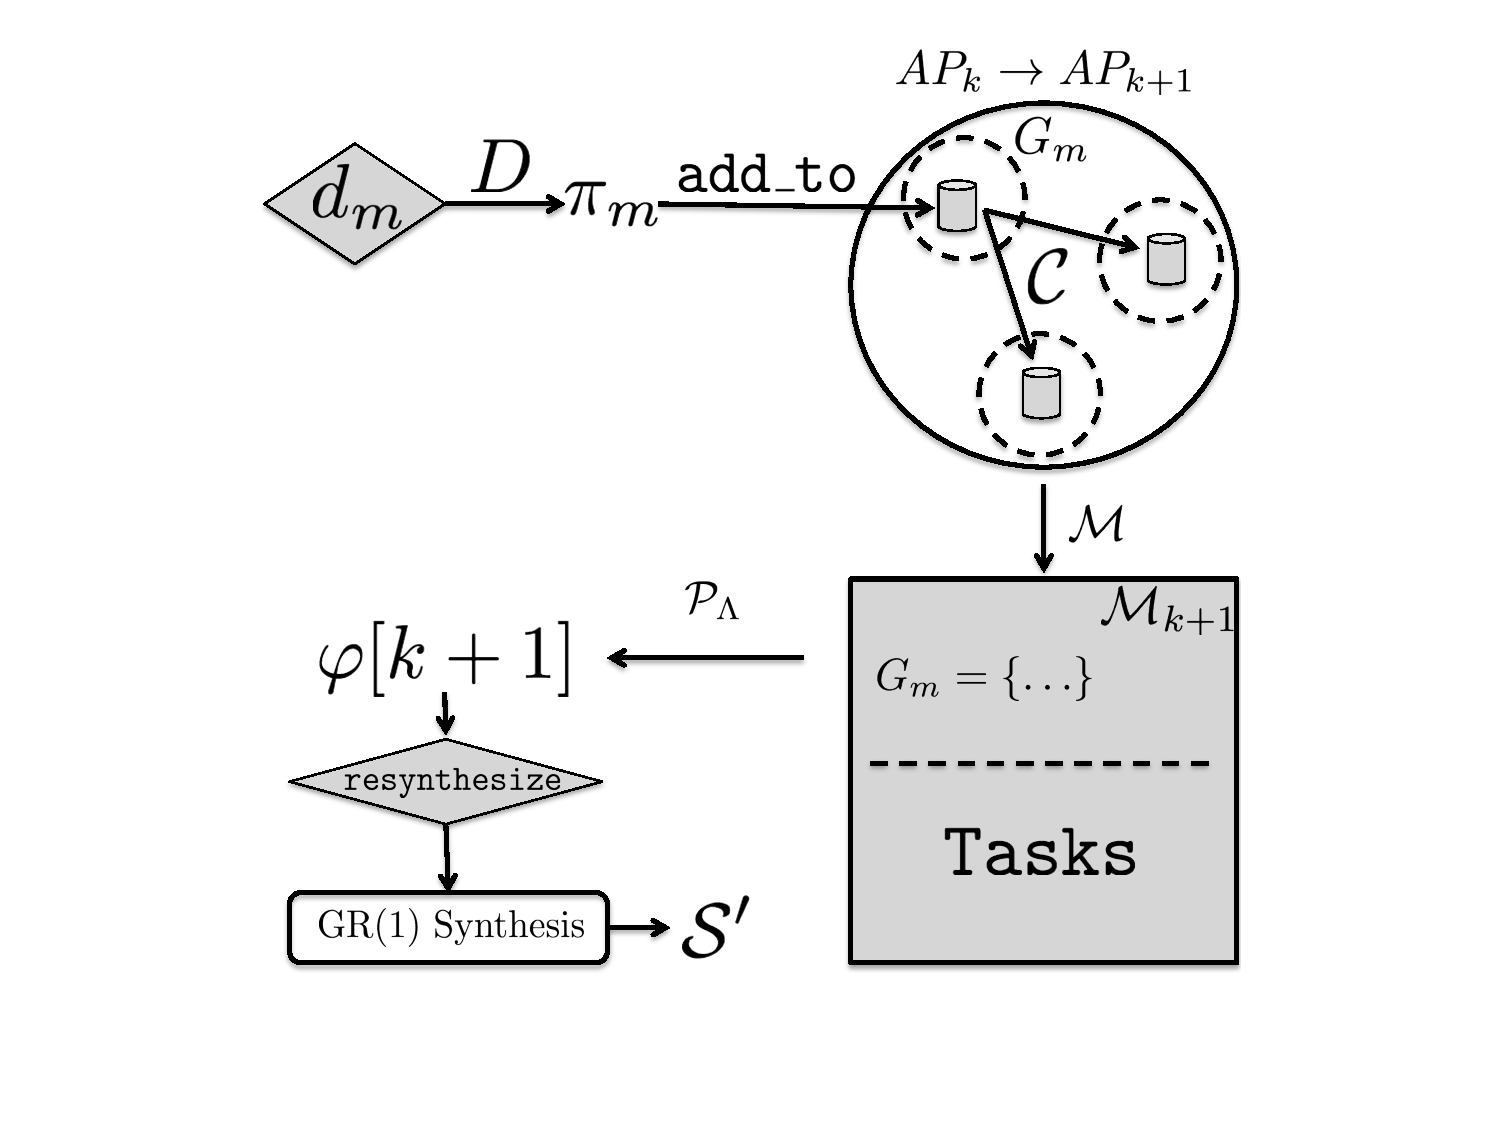
\includegraphics[width=0.9\columnwidth, clip]{./img/approach.pdf}
	\caption{Illustration of our approach, where, for clarity, a single new proposition $\pi_{m}$ is added to a single group $G_m$, i.e., $\texttt{add\_to}(\pi_{m}, G_m)$.} % TODO: Write stuff here
	\label{Fig:approach}
\end{figure}
% END

\section{SIMULATION IN LTLMOP}\label{simulation}  % or make exploration a subsection in pref section
We implemented the proposed approach to open-world mission specification in LTLMoP (the Linear Temporal Logic Mission Planning toolkit; see Section \ref{preliminariesB}). We augmented Structured English, one of LTLMoP's available specification languages, with \emph{open-world abstractions} (groups, quantifiers, and correspondences), the \emph{add to group} operator, and a \emph{resynthesis} action.

\begin{myExample}\label{Ex:mailbot3} We revisit the mailbot scenario from Examples \ref{Ex:mailbot1} and \ref{Ex:mailbot2}, and present the full mission specification, $\mathcal{M}_0$. The robot's workspace is depicted in Fig. \ref{Fig:map}.
\end{myExample}

Initially, the robot has no information about specific letters or their recipients. Therefore, it patrols the regions in \texttt{PatrolRooms}. If it senses a new letter, it will add a proposition to the group \texttt{Letters}. In simulation, LTLMoP prompts the user for the name of the proposition, e.g. \texttt{letter1}. Additionally, the \emph{add to} operator has to add a proposition to the group \texttt{Offices}, in order to maintain the correspondence. LTLMoP prompts the user a second time, and he inputs one of the region names, \texttt{r1}--\texttt{r6}. The two user prompts simulate the process of scanning the letter for the recipient's name and address, in order to name and ground the new propositions (see Assumption \ref{Ass:grounding}).

\begin{algorithm}
	\textbf{Mission specification:} Autonomous Mailbot
	
	\vspace{-7 pt}
	\hrulefill\\
	{\small
	
	\textbf{Group declarations:}\\
	\texttt{Group Letters is empty} \\
%	\texttt{Group LetterSlots is empty} \\
%	\texttt{Group Delivery is empty} \\
	\texttt{Group Offices is empty} \\
	\texttt{Group PatrolRooms is mailRoom, hallW, hallN}\\ % FIXME: I don't like 'hall_x"s
	
	\textbf{Correspondence definitions:} (immutable)\\ %FIXME: Add more for add_to to work?
%	\texttt{Letters correspond to LetterSlots, Delivery, Offices}\\ %FIXME: This isn't implemented
%	\texttt{LetterSlots correspond to Letters}\\
%	\texttt{LetterSlots correspond to Delivery}\\
%	\texttt{Delivery correspond to LetterSlots}\\
%	\texttt{Delivery correspond to Offices}\\
	\texttt{Letters correspond to Offices}\\
	
%	\hrulefill\\
	% TODO: We can't have initial conditions when we are re-synthesizing, right?
%	\textbf{Initial conditions} (optional)\\
%	\texttt{Robot starts in mailRoom with false}\\
%	\texttt{Environment starts with false}\\
	
	\textbf{Mission tasks:} (immutable)\\
	\texttt{If you are sensing any Letters then go to the corresponding Office}\\
	\texttt{If you are not sensing any Letters then visit each PatrolRoom}\\
%	\texttt{Each LetterSlot is set on the corresponding Letter and pickUp and reset on the corresponding Delivery}\\
	
%	\texttt{Do pickUp if and only if you are sensing any Letters}\\
%	\texttt{If you are activating pickUp then stay there}\\
	
%	\texttt{Do each Delivery if and only if you are in the corresponding Office and you are activating the corresponding LetterSlot}\\
	
%	\texttt{Infinitely often not each LetterSlot}\\
%	\texttt{If you are not activating any LetterSlots then visit each PatrolRooms}\\
	
	\textbf{Open--World settings:} (immutable)\\
	\texttt{If you are sensing newLetter then add to group Letters and resynthesize}\\
	\texttt{If you are sensing newLetter then stay there}\\
		
	\textbf{Environment fairness assumption:} (immutable)\\
%	\texttt{Infinitely often not any Letters}\\
	\texttt{Infinitely often not newLetter}\\
	}
	\vspace{-10 pt}
\end{algorithm}

\begin{figure}[h]
	\centering
	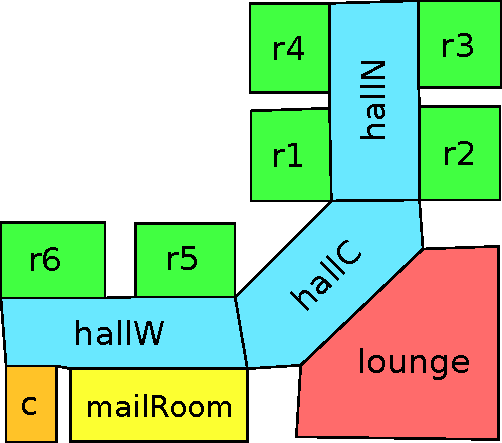
\includegraphics[width=0.80\columnwidth, clip]{./img/mailbot_map.pdf}
	\caption{Map of workspace for mailbot scenario.  Regions \texttt{r1}--\texttt{r6} are the offices of potential letter recipients.} 
	\label{Fig:map}
\end{figure}

After the specification is rewritten, the LTL formula $\varphi [k]$ changes to $\varphi [k+1]$, according to Eqs. \eqref{Eq:newSpecA} and \eqref{Eq:newSpecB}. The change involved adding a new mission goal: the delivery of \texttt{letter1} to the corresponding office \texttt{r1}. Specifically, compared to $\varphi_g^s [k]$, $\varphi_g^s [k+1]$ contains the additional liveness requirement:
\begin{equation*}
	\G\F\left( \texttt{letter1} \Rightarrow \texttt{r1} \right)
\end{equation*}

After resynthesis, the robot can now sense letters in two ways. First, it could detect a letter addressed to the same recipient as \texttt{letter1}. In this case, \texttt{letter1} will become \texttt{True}, and the robot will deliver the letter to \texttt{r1}. Second, it could detect a letter addressed to a new recipient. In that case, the sensor \texttt{newLetter} will become \texttt{True}, and the \emph{add to group} operator will once again cause new propositions to be added to \texttt{Letters} and \texttt{Offices}.

% END
%
%\begin{myExample}\label{Ex:restaurant} Robotic Waiter \\
%	Overview of task \ldots
%\end{myExample}
%
%\begin{algorithm}
%	\textbf{Mission specification:} Robotic Waiter\\
%	{\small
%	\texttt{Group Customers is empty}\\
%	\texttt{Group Orders is empty}\\
%	\texttt{Group ... is empty}\\
%	\texttt{Group ... is empty}\\
%	
%	\texttt{Orders correspond to Customers}\\
%	\texttt{... correspond to...}\\
%	
%	\texttt{if you are activating any Orders then go to kitchen and do corresponding FoodPickUp and go to corresponding Customer and do corresponding ServeFood}\\
%	\texttt{...}\\
%	
%	\texttt{...}\\
%	}
%	
%	\textbf{Open World Settings:}\\
%	{\small
%	\texttt{if you are sensing newOrder then add to Orders}\\ % TODO: ... and add to corr. groups?
%	\texttt{...} 
%	}
%\end{algorithm}
%
%\begin{myExample}\label{Ex:planetxplore} Autonomous Planetary Exploration\\
%	Consider now the more futuristic scenario of autonomous planetary exploration using rovers. In order to lessen the dependency of the rover from the engineers on Earth, the rover will be given a mission specification that it should carry out autonomously. However, the need to redefine the mission will arise as the rover discovers interesting elements of its environment, such as new types of rock and regions interest. In these cases, the engineers and scientists on Earth should be able to extend the rover's mission specification without sacrificing correctness or rewriting the specification from scratch.
%	
%	Specifics: exploration, new stuff sensor, new requests.
%\end{myExample}
%
%\begin{algorithm}
%	\textbf{Mission specification:} Autonomous Planetary Exploration\\
%	{\small
%	\texttt{Group InterestingRegions is empty}\\
%	\texttt{Group PendingRequests is empty}\\
%	\texttt{Group Sites is empty}\\
%	\texttt{Group Actions is empty}\\
%	
%	\texttt{Sites correspond to Requests}\\
%	\texttt{Actions correspond to Requests}\\
%	
%	\texttt{Recharging is set on BatteryLow and reset on BatteryFull}\\
%	\texttt{if you are activating Recharging then stay there}\\
%	\texttt{infinitely often BatteryFull}\\
%	
%	\texttt{visit each InterestingRegion and do Panorama}\\
%	\texttt{if you are activating any PendingRequests then go to the corresponding Site and do the corresponding Action}\\
%	\texttt{each PendingRequest is toggled on the corresponding Site and the corresponding Action}\\
%	}
%	
%	\textbf{Exploration Settings:}\\
%	{\small
%	\texttt{do exploreMODE if and only if you are not activating Recharging}\\
%	\texttt{if you are sensing newInterestingRegion then add to InterestingRegions}\\
%	\texttt{...} 
%	}
%\end{algorithm}
%
%\begin{figure}[h]
%	\centering
%	\includegraphics[width=0.7\columnwidth, clip]{./img/planetXplore_regions.pdf}
%	\caption{Workspace for the autonomous planetary exploration scenario (to be updated and broken down to intermediate exploration steps).}
%	% TODO: Update this map. Regions should be around the land site! No mountain next to it either.
%	% Instead of the final map, show intermediate steps as the workspace is expanded.
%	\label{Fig:planetxplore}
%\end{figure}

\section{CONCLUSIONS AND FUTURE WORK}\label{conclusion}
%\addtolength{\textheight}{-14 pt}   % This command serves to balance the column lengths
                                  % on the last page of the document manually. It shortens
                                  % the textheight of the last page by a suitable amount.
                                  % This command does not take effect until the next page
                                  % so it should come on the page before the last. Make
                                  % sure that you do not shorten the textheight too much.
In this paper, we presented an approach to specifying and updating robot missions that take place in worlds open with respect to new elements, such as new objects and regions of interest. During execution, the new elements are translated into new propositions, which are automatically incorporated into the mission specification. This is possible via (i) \emph{open-world abstractions}, which enable us to specify high-level behaviors without explicitly referring to individual propositions, and (ii) the \emph{add to Group} mechanism, which systematically augments sets of propositions with new elements. A notable advantage of our approach is that it allows the user to specify how the new elements will be incorporated into the mission, and under which conditions the updates will be reflected in the robot's controller.

%The open-world model defined in this paper is strictly expanding, i.e., it only permits the addition of propositions. 
A future research direction is the generalization of our model in order to also account for the removal of propositions that are no longer pertinent to the mission. 
In addition, our method of translating an updated specification to a new execution strategy is that of global resynthesis. We will investigate \emph{local} resynthesis approaches, in the direction of \cite{MurrayICRA2012, MurrayICRA2013a}.
The ability to remove propositions, coupled with the efficiency of local resynthesis will allow us to deal with large-scale open worlds without synthesis becoming a computational bottleneck.
Furthermore, we intend to generalize and formalize the introduction of elements of first-order logic to our specification language.
%Furthermore, we will explore the use of additional first-order logic elements, in order to enhance the expressivity of our mission specifications.
On the implementation side, we are interested in a human-robot dialogue interface that would allow users to specify new tasks during execution.
%Finally, we would like to apply our approach to modular robots \cite{ModularIROS2011} with the ability to assimilate new components found in the open world to extend their functionality on-the-fly.
% END

%\addtolength{\textheight}{-12cm}   % This command serves to balance the column lengths
                                  % on the last page of the document manually. It shortens
                                  % the textheight of the last page by a suitable amount.
                                  % This command does not take effect until the next page
                                  % so it should come on the page before the last. Make
                                  % sure that you do not shorten the textheight too much.

%%%%%%%%%%%%%%%%%%%%%%%%%%%%%%%%%%%%%%%%%%%%%%%%%%%%%

%\section*{APPENDIX}
%
%...

\section*{ACKNOWLEDGMENT}

The authors would like to thank Cameron Finucane for insightful discussions and for his contributions to the implementation of the proposed approach in LTLMoP.

%%%%%%%%%%%%%%%%%%%%%%%%%%%%%%%%%%%%%%%%%%%%%%%%%%%%%

\bibliographystyle{ieeetran}
\bibliography{spyros-biblio,matt-biblio}

\end{document}
